\chapter{Bound diffusion measurements}\label{ch04}
\label{ch:bound-diffusion}

Following up on the principles of the bound-diffusion theory, we wanted to see whether we could measure bound diffusion in a biomaterial inspired by the nuclear pore complex.  In order to do that, we made Nup-filled hydrogels and measured the diffusion of transport factors and inert proteins within them.  We measured the diffusion in a few different ways: monitoring the concentration profile and total accumulation as the proteins diffused into the cell, and using fluorescence recovery after photobleaching (FRAP).

Fluorescence recovery after photobleaching (FRAP) relies on the redistribution of fluorophores after patterned photobleaching in order to determine their diffusion constant.  After a small portion of the hydrogel is bleached, the bleached spot gradually exchanges with the non-bleached fluorophores outside, and the average fluorescence intensity within the bleached spot recovers.  The recovery lifetime can be used to determine the fluorophore's diffusion constant, and the final recovered intensity as compared to the intensity outside the bleach spot can be used to determine the mobile fraction of fluorophore.

\section{Experimental parameters}

Our reaction-diffusion model of selectivity is controlled by a relatively small number of parameters.  Ideally, we would like to vary all of these experimentally in order to verify the model's predictions.  In reality, most are highly difficult to alter in a well-controlled way.  Of the model's parameters, the contour length $L_C$ of the tethered Nups is the simplest to control.  Varying this contour length will very the bound diffusion coefficient $D_B$ according to Eqn.~\ref{eq:dbound}.  This section discusses $L_C$ and the other experimental parameters used in our hydrogel nuclear pore mimics.

\subsection{Nup contour length and valency}

The most straightforward way to vary $D_B$ is to change the contour length of the Nups that are anchored into the hydrogel.  To that end, we compared hydrogels containing the constructs FSFG concat-1 and FSFG concat-2 (Sec.~\ref{sec:Nups}, Appendix~\ref{appx:sequences}).  These Nup fragments have $L_C = 50$ nm and 100 nm, respectively.  Given the parameters described below, the bound diffusion constant should increase by roughly 40\% from FSFG concat-1 to FSFG concat-2.

In addition to differing lengths, the FSFG concat-1 and concat-2 differ in their number of binding sites, with six and twelve respectively.  In order to control for the change in binding valency, we tested FSFG concat-2 hydrogels with the same molar concentration of FG repeats as the FSFG concat-1 gels as well as testing gels with the same molar concentration of Nups.

\subsection{Binding affinity of NTF2 and FSFG}
% ITC data is in book 1, a bit of book 2.  None of the fits were good.  Data shown here is taken from the runs on 6/18/14 and 6/23/14.  Fits aren't shown because we never really understood them.
Although bound diffusion is the key parameter from our reaction-diffusion model of selectivity, the kinetic parameters of off-rate $\koff$, on rate $\kon$, and dissociation constant $K_D = \koff/\kon$ are also important. These parameters are surprisingly difficult to measure, yielding values between 10 nM and 10 $\mu$M depending on the experimental conditions.  We estimated the dissociation constant for NTF2 and FSFG concat-1 using isothermal titration calorimetry (ITC).  The heat of injection was recorded as FSFG was titrated into a stock of NTF2.  While the resulting titration curves had low signal-to-noise and did not reach saturation, they clearly indicated binding (Fig.~\ref{fig:ITC-runs}).  Simple fits are likely inaccurate, given the high degree of multivalent binding, but may provide an order-of-magnitude estimate of the affinity.  Several ITC curves agree on a dissociation constant of $K_D \approx 200 \mu$M.  This is roughly compatible with the millimolar per-FSFG constant measured by the Rout lab with NMR and ITC \cite{hayama18}.  Similarly weak values were predicted through NMR, simulation, and stopped-flow anisotropy \cite{milles15}.

\begin{SCfigure}
\caption{Isothermal calorimetry titration curve: heat of injection vs. molar ratio of FSFG to NTF2. Fits are questionable but multiple runs suggest $K_D \approx 200\ \mu$M.\\}
\centering
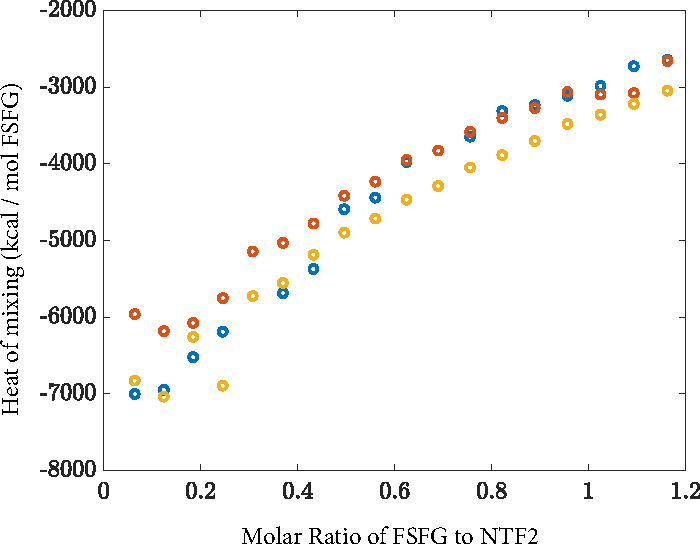
\includegraphics[width=0.6\textwidth]{figs/ch04/ITC_runs}
\label{fig:ITC-runs}
\end{SCfigure} 

Due to the twin difficulties of varying $K_D$ in a controlled way and accurately measuring its value, we did not attempt to experimentally alter this parameter.  Ideally, a transport factor - Nup pair with $K_D \approx 1 \mu$M would have been used to maximize selectivity.  For the purposes of determining the bound diffusion constant, the only value that is necessary to measure is the ratio $K_D/N_T$, which can be estimated using the partitioning of transport factors and inert proteins into the FSFG hydrogels (Sec.~\ref{sec:part-coeff}).  We investigated using the ubiquitin-associated (UBA) domain of the mRNA exporter Mex67 as a Nup-binding domain in GFP fusion proteins.  In principle, varying numbers of this small ($<$10 kDa) domain could be added to GFP to explore the effect of varying binding affinity and valency in transport factors.  The constructs GFP-UBA, GFP-UBAx2, and GFP-UBAx3 were created by Eric Verbeke, but did not express and/or bind well.

%Eric did most of the UBA cloning I think
% Expression tests in LKM book 5 pgs 146-9

\subsection{Quantifying concentration of tethered Nups}

Another potentially-tunable parameter of the bound-diffusion model is $N_T$, the total concentration of tethered Nups.  It is straightforward to control the Nup concentration in the hydrogel precursor solution by resuspending a known mass of lyophilized proteion.  Nup concentrations up to $\sim 50$ mg/mL can be resuspended.  However, it is much more difficult to determine how much protein was tethered to the hydrogel upon crosslinking. 

 BCA protein quantitation assays were used to place upper bounds on $N_T$.  Two methods were attempted: incubating the hydrogel itself in the working reagent, and soaking the hydrogel in a known volume of buffer and testing the concentration of FSFG released.  When applying the first method, the hydrogel was first soaked to remove excess precursor solution and thoroughly rinsed.  The gel was placed into a 96-well plate and buffer added until the appropriate sample volume was reached.  A standard BCA protocol was then followed.  Upon incubation with the working reagent, the hydrogels turned purple, as expected.  Standard absorption measurements and processing yielded an estimate of 0.5 mg/mL tethered FSFG-concat 1; this should be taken as an approximate value only.  The second method, that of soaking hydrogels and measuring the FSFG released, placed a similarly-low upper bound on tethered FSFG concentration.  Hydrogels made with 5 $\mu$L of precursor solution were soaked in 45 $\mu$L buffer to equilibrate.  The buffer was then measured to have a concentration of 1.0 mg/mL FSFG, implying a tethered FSFG concentration of $<1$ mg/mL.
% LKM book 5 pgs 119 and later

The concentration of Nups within the pore may reach 100 mg/mL \cite{thing}.  The low concentration of tethered Nups that we were able to achieve is therefore a major barrier to selectivity.  It is likely that the disordered nature of FSFG makes the labeled end less accessible to the hydrogel scaffold than would be the case for an ordered protein.  In an effort to overcome this limitation, we tested other linkers and conjugation methods.  We conjugated the FSFG-cys to PEG-diacrylate of varying lengths (700 Da and 10 kDa), to multi-armed PEG-diacrylate, and to maleimide-PEG-acrylate.  While labeling was verified using Ellman's reagent (Appendix~\ref{appx:bis-labeling}), there was no noticeable difference in transport factor partitioning into these hydrogels.
% maleimide-PEGDA LKM book 6 pgs 7-10
% multi-armed PEGDA LKM book 5 pg 151
% basic PEGDA conjugations throughout book 5

\subsection{Free diffusion constant}

The final tunable parameter from the binding-diffusion model is the diffusion constant of the transport factor when it is not bound to a Nup, the free diffusion constant $D_F$.  Decreasing $D_F$ is predicted to increase a material's selectivity while decreasing the absolute flux of transport factor (Figs.~\ref{fig:parameter-variations}, \ref{fig:parameter-variations-abs-flux}).  The free diffusion is predominantly determined by the protein's size and the viscosity of the solution, according to the Stokes-Einstein equation $D = k_BT/6\pi\eta R$, where $k_BT$ is the thermal energy, $\eta$ the solution viscosity, and $R$ the particle radius.  The solution viscosity could potentially be increased using a viscous additive such as glycerol; however, these attempts appeared to interfere with the binding of NTF2 and FSFG.

The diffusion of the non-binding 30 kDa protein mCherry was used as a proxy for the free diffusion of similarly-sized NTF2 within the FSFG hydrogels.

\section{Experimental procedures}

The nuclear pore mimics in this dataset were designed with the lessons of Chapter~\ref{ch03} in mind.  They consist of hydrogels with the largest average pore size and simplest geometry: a single microliter-scale droplet.  While this geometry does not allow for direct measurements of selectivity, the in-gel diffusion constants of both NTF2 and mCherry can be determined and bound diffusion calculated.  Two types of experiments were carried out: influx experiments, in which the entry of fluorescent proteins into the hydrogels was monitored, and FRAP experiments, in which a portion of an equilibrated hydrogel was bleached and the recovery observed.  Both experiments provide a measurement of the proteins' diffusion constants.  These experiments were performed at CU's BioFrontiers Advanced Light Microscopy Core Facility.  Thanks go to Joseph Dragavon for much assistance with the microscopy.

\subsection{Hydrogel preparation}

Detailed precursor solution recipes are given in Appendix~\ref{appx:precursor-recipes}.  For the dataset analyzed in this chapter, all nuclear pore mimic hydrogels were 6\% acrylamide and contained 2 mM LAP.  The precursor was made with potassium transport buffer (PTB) and contained either FSFG concat-1 bis or FSFG concat-2 bis.  Lyophilized FSFG-bis was resuspended in PTB, allowed to sit at room temperature for at least 20 minutes, and added to the precursor solution.  After the precursor solution was thoroughly mixed, it was degassed in a vacuum desiccator for 10 minutes and immediately pipetted into a disassembled 400-$\mu$m-thick PDMS gasket chamber (Sec.~\ref{sec:gel-geometries}).  Drops between 0.5 and 2 $\mu$L were carefully pipetted onto the plastic slide and the chamber assembled around the drops.  Typically, each chamber measured a few centimeters on a side and contained a control gel with no Nups as well as one or more Nup-filled gels.  The chamber was then illuminated as uniformly as possible with 365 nm light at approximately 200 mW/cm$^2$ with a ThorLabs M365 LP1 LED.  Condensation around the gels indicated that they had crosslinked.  The chamber was immediately rinsed with at least 100 $\mu$L of PTB, filled with fresh PTB, and sealed with a PDMS slab and clingwrap.  The gels were left to soak at 4$^\circ$C for at least 12 hours so that any remaining precursor solution and protein could leave the gel.

\subsection{Influx of transport factor and inert protein}
After soaking in buffer, the buffer solution was removed by pipette or wicking with a Kimwipe and a fluorescent reservoir solution added.  Aspirating the chamber was avoided if possible, as it sometimes disturbed the seal between the gel and the chamber.  The reservoir solution contained 20 $\mu$M each freshly-thawed NTF2-fluorescein (NTF2-F) and mCherry in PTB.  The chamber was resealed after adding the solution.  If no influx experiment was planned, the gels were then allowed to  equilibrate for 24 hours before FRAP was performed.

When influx experiments were run, they began as soon as possible after loading the reservoir solution.  Videos were recorded at 4x magnification on an Olympus IX-81 widefield microscope using FITC (excitation 464-500 nm / emission 516-556 nm) and TRITC (excitation 532-544 nm / emission 573-613 nm) filter cubes.  Exposure times were typically 30-100 ms with 3-8 dB gain.  Videos consisted of 120 frames at one frame per minute. Minimal photobleaching took place over the course of these experiments.  After the influx experiment, the chamber was usually stored for equilibration 4$^\circ$C, protected from light, and a FRAP experiment performed the following day.

Influx experiments on hydrogels containing FSFG show binding of NTF2-F to mCherry (Fig.~\ref{fig:influx-images}).  A bright wavefront  of NTF2-F slowly progresses into the gel, while mCherry remains largely excluded.  As expected, mCherry equilibrates more rapidly than does NTF2-F, due to the lack of binding.  Influx experiments were analyzed as described in Sec.~\ref{sec:influx-analysis}.

 % '/Volumes/houghgrp/Processed Images/2019-2-21_5/results.mat'
%'/Volumes/houghgrp/Microscopy/190220/190220_profiles_02.vsi’
%Cct2
%grnScale = [0;0.07];
%redScale = [0.0183566033417258;0.0502479591058213];
%Image_series_figures.m
\begin{figure}
\caption{Influx image series.  A hydrogel containing a nominal 5 mg/mL FSFG concat-2 was challenged with 20 $\mu$M NTF2-F and mCherry.  The hydrogel shows selective entry of NTF2-F and has largely equilibratd within 24 hours.}
\centering
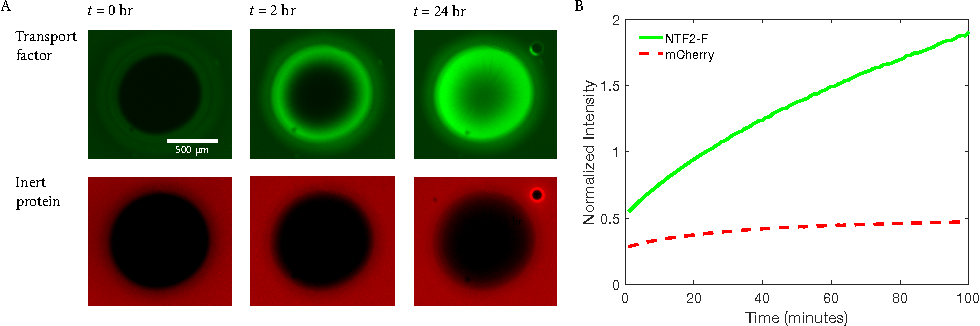
\includegraphics[width=0.9\textwidth]{figs/ch04/influx-images-clean.pdf}
\label{fig:influx-images}
\end{figure} 

\subsection{Fluorescence recovery after photobleaching}

FRAP is typically performed using a confocal microscope, but we were able to bleach the hydrogels using an Olympus IX-81 widefield microscope.  The widefield was preferable because the greater depth of field allowed for thicker hydrogel samples, which were easier to fabricate and manipulate.  As described above, the hydrogel was first allowed to equilibrate with 20 $\mu$M NTF2-F and mCherry in PTB.  A reference image was taken at 4x magnification in both fluorescence channels.  A circular region of the hydrogel around $300 \mu$m (?? check this) in radius was then photobleached by taking a five-second exposure at 40x magnification using a DAPI (excitation 352-402 nm / emission 417-477 nm) filter cube.  Following the bleach, the 4x objective was rapidly returned and a time series recorded.  Typical series consisted of 15-30 frames taken as rapidly as possible (5-10 s per frame), followed by 30-60 frames taken at a slower rate (1-2 minutes per frame).  Total experiment time was 1-4 hours.  Typical exposure times were 10 ms for NTF2-F and 40 ms for mCherry, both with a gain of 3 dB.

In order to increase throughput, up to three FRAP experiments were run concurrently by sequentially bleaching and then imaging several locations within a single chamber.  This led to a maximum delay time of approximately 35 s between the end of the bleach segment and the beginning of the time series.  Delay times were recorded and taken into account in the data processing. Figure~\ref{fig:frap-images} shows a representative series of images pre- and post-FRAP for both NTF2-F and mCherry.

Despite allowing 24 hours for equilibration, the fluorescence intensity across the hydrogel was not always uniform at the beginning of a FRAP experiment.  This could be due to slow diffusion into the hydrogels, or to inhomogeneous crosslinking.  The center of a hydrogel is more likely to be tightly crosslinked than the edges, as swelling is most inhibited at the center.  Gels which were too inhomogenous to display a clear bleach spot were discarded, but many nonuniform hydrogels were used in the final dataset, with the lack of equilibrium addressed in the data analysis (Sec.~\ref{sec:FRAP-analysis}).  Smaller hydrogels (0.5 $\mu$L of precursor solution) equilibrated more readily, at the cost of increasing the effect of fluorescent protein exchange with the reservoir, since the bleach spot then covered a significant fraction of the hydrogel.  This effect was also taken into account during data analysis.

% 2019-2-19, #21
%Cct1
%'/Volumes/houghgrp/Processed Images/2019-2-19_21/results.mat'
%[0.005;0.0222781719691768]
%Both scales
%Image_series_figures.m
\begin{figure} 
\caption{FRAP image series. NTF2-FITC (top, green) and mCherry (bottom, red) bleaching and recovery shown separately.  Hydrogel contained... }
\centering
\includegraphics[width=\textwidth]{figs/ch04/FRAP-images.pdf}
\label{fig:frap-images}
\end{figure} 

\section{Steady-state hydrogel properties}

Both the influx and FRAP experiments rely on steady-state properties of the hydrogel as well as time-dependent ones.  These properties include the partition coefficients of transport factors and inert proteins, as well as some dependent on the geometry of the hydrogel.

\subsection{Gel dimension estimates}
\label{sec:gel-dim}

% Hydrogel 19-2-6-21, grnScale [0.0;0.03], redScale [0.01;0.06], cropping rect 155.51 	0.51	1069.98 1023.98
\begin{SCfigure} 
\caption{Sample hydrogel mask with radius and center calculations.  (A) An equilibrated hydrogel containing FSFG concat-1, immediately post-bleach. (B) The corresponding hydrogel mask (white), bleach spot mask (light gray), calculated gel diameter, and calculated gel center.}
\centering
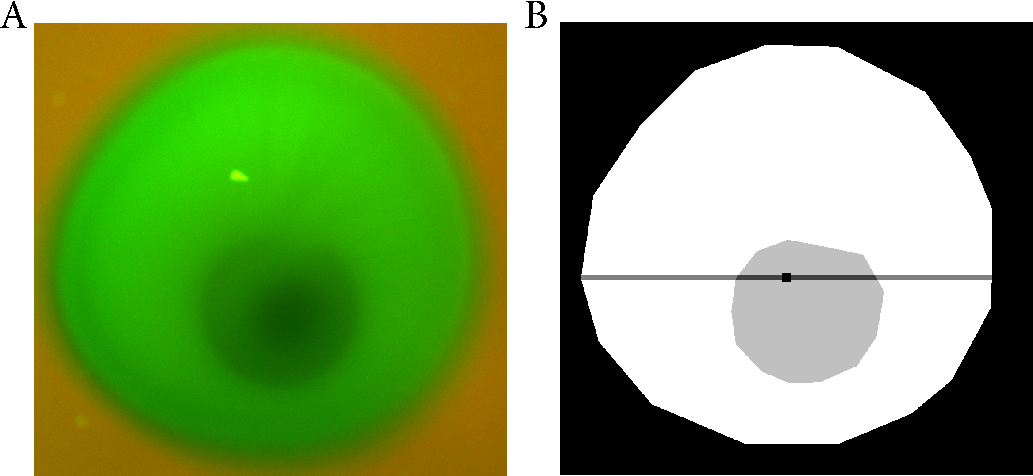
\includegraphics[width=0.5\textwidth]{figs/ch04/geometry.pdf}
\label{fig:masks}
\end{SCfigure} 

Although the hydrogels were not perfectly circular, all analysis treated them as circular or nearly so.  In total, the analysis made use of a gel's radius, center, perimeter, and area.  I began by manually defining two masks: one that covered the entire gel, and one that covered only the bleach spot (Fig.~\ref{fig:masks}).  The gel area was calculated by summing all of the pixels in the gel mask and, where necessary, making use of the 1.58 $\mu$m per pixel scale of the Olympus 4x objective.  The perimeter was calculated using Matlab's \texttt{bwperim} function, which takes a binary mask and returns a mask whose only nonzero entries are that mask's perimeter.  Summing over these pixels and scaling provides the gel perimeter.  It should be noted that in some cases the full area of the gel was not within the field of view.  In these cases, sometimes the partial area in the field of view was used as the area estimate, and sometimes I embedded the gel image in a larger frame and estimated the remaining area when drawing the mask.  Following sections indicate which method was used and the mathematical reasoning.  However, all perimeter calculations were performed with the estimated full area.

The hydrogel radius was estimated taking the diameter to be the widest row of the gel mask.  The widest row also set the y-coordinate of the gel center, with the x-coordinate calculated to be midway along the non-zero values for that row.  As seen in Fig.~\ref{fig:masks}, this is a quick and relatively crude method, but in almost all cases it works reasonably well.  An advantage of this method is that it works even for hydrogels which do not fit in the vertical field of view.

\subsection{Partition coefficients and fraction of time spent bound}
\label{sec:part-coeff}

% Hydrogel 19-2-6-21, grnScale [0.01;0.03], redScale [0.01;0.06], cropping rect 155.51 	0.51	1069.98 1023.98
\begin{SCfigure} 
\caption{Partitioning of NTF2 and mCherry into FSFG hydrogel.  (A) Partition coefficient $\gamma$ depends on whether the hydrogel excludes or binds protein. (B) Equilibrated FSFG concat-1 hydrogel (nominally 10 mg/mL) showing partitioning of $T_L = 20\ \mu$M each NTF2-FITC and mCherry.  Contrast adjusted for ease of viewing.\\}
\centering
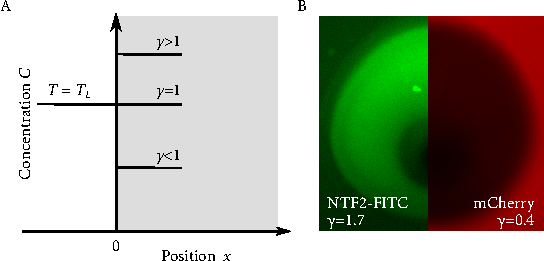
\includegraphics[width=0.6\textwidth]{figs/ch04/partition.pdf}
\label{fig:partition}
\end{SCfigure}

The concentration of NTF2 and mCherry in a flow chamber's reservoir can be directly controlled, but the partitioning of a protein into the hydrogel depends on the degree to which the presence of the gel sterically excludes the protein, as well as on binding interactions between the gel and protein.  When a transport-factor-sized inert protein is present to control for the steric effects, information about the transport factor's dissociation constant and fraction of time spent bound can be extracted from knowledge of the partition coefficient $\gamma$.  In particular, $p_B$, the fraction of time spent bound, is necessary in order to calculate the bound diffusion coefficient.

As shown in Fig.~\ref{fig:partition}A, the partition coefficient is the ratio of a protein's concentration in a well-equilibrated hydrogel to that in the surrounding reservoir.  This quantity is calculated by dividing the average intensity of the gel by that of the reservoir within the field of view (Fig.~\ref{fig:partition}B).  If the gel is not fully equilibrated, the partition coefficient can be estimated using a line scan through the reservoir and gel, though this will likely underestimate the true value.

When the system is in chemical equilibrium, the concentration of free transport factor ($T$), free Nup ($N$), and transport factor - Nup complex ($C$) is related to the dissociation constant $K_D$ by
%\begin{equation}
%K_D = \frac{TN}{C}
%\label{eq:chem-equil}
%\end{equation}
$K_D = NT/C \approx N_TT/C$ in the linear approximation $N \approx N_T$.   The total tethered Nup concentration, both free and bound, is the constant $N_T$.  The fraction of transport factors that are bound is then given by
\begin{equation}
p_B = \frac{C}{C+T} = \frac{C}{C+\frac{CK_D}{N_T}} = \frac{1}{1+\frac{K_D}{N_T}} %\approx 1 - \frac{K_D}{N_T}
\label{eq:bound-prob}
\end{equation} %where the final step applies if $K_D \ll N_T$, which might be the case but now I'm confused again.

To relate this expression to measureable quantities, write the protein concentrations within the hydrogel in terms of their partition coefficients. The concentration $c_0$ of the inert protein and the transport factor is equal in the reservoir.  If $\gamma_T$ is the partition coefficient of the transport factor and $\gamma_I$ that of the inert protein, then the transport factor concentrations can be expressed as
\begin{eqnarray}
T &=& \gamma_I c_0\\
C & =& T_T - T = \gamma_Tc_0 - \gamma_I c_0
\label{eq:gamma}
\end{eqnarray} 
The total transport factor concentration within the gel is $T_T = T + C$ and is a constant.
Therefore, within the gel, the chemical equilibrium condition can be expressed as
\begin{equation}
\frac{K_D}{N_T} = \frac{T}{C} = \frac{\gamma_I c_0}{\gamma_T c_0 - \gamma_I c_0} = \frac{\gamma_I}{\gamma_T - \gamma_I}
\label{eq:partition}
\end{equation}
Combining Eqns.~\ref{eq:bound-prob} and \ref{eq:partition}, the bound probability can be expressed in terms of the partition coefficients as
\begin{equation}
p_B= \frac{1}{1+\frac{K_D}{N_T}} = \frac{1}{1+\frac{\gamma_I}{\gamma_T - \gamma_I}} = 1 - \frac{\gamma_I}{\gamma_T}
\label{eq:bound-prob-final}
\end{equation}

\subsection{Bound-diffusion calculation}

Once the observed diffusion constants for NTF2 and mCherry have been calculated, along with the fraction of time spent bound $p_B$, the bound diffusion is given straightforwardly by the weighted average
\begin{equation}
D_\mathrm{obs, TF} = p_B D_B + (1-p_B) D_F
\label{eq:weighted-average}
\end{equation}
This result assumes Fickian diffusion.  In reality the diffusion will be slightly anomalous due to binding and the presence of the hydrogel.  However, the binding is highly transient and the hydrogel relatively permeable to proteins of the size of NTF2 and mCherry (Sec.~\ref{sec:pore-size}).

Taking the free diffusion coefficient of the transport factor to be approximately equal to the observed diffusion of the inert protein ($D_F = D_\mathrm{obs,I})$, the bound diffusion coefficient of the transport factor is
\begin{equation}
D_B = \frac{D_\mathrm{obs, TF}-(1-p_B) D_\mathrm{obs,I}}{p_B}
\label{eq:d-bound}
\end{equation}

Note that neither the dissociation constant or the total Nup concentration need to be measured independently in order to calculate the bound diffusion constant.

\section{Influx analysis}
\label{sec:influx-analysis}

%2/20/19 #2 , also 2-21-19 #5 first image, grn scale [0.0038; 0.023], red [0.00; 0.0381], crop rect [3.915100000000000e+02,1.755100000000000e+02,8.259800000000000e+02,7.979800000000000e+02]
\begin{figure}
\caption{Intensity profiles and total accumulation within hydrogel as determined from influx time series.  (A) Image of an FSFG concat-2 hydrogel with a nominal Nup concentration of 10 mg/mL. Reservoir contains 20 $\mu$M NTF2-F and mCherry in PTB. Reservoir mask is shown (red polygon) as well as accumulation area and rectangle over which the profile averaging was performed. (B) Normalized intensity profiles as calculated using the box in (A).  (C) Normalized average intensity within hydrogel.}
\centering
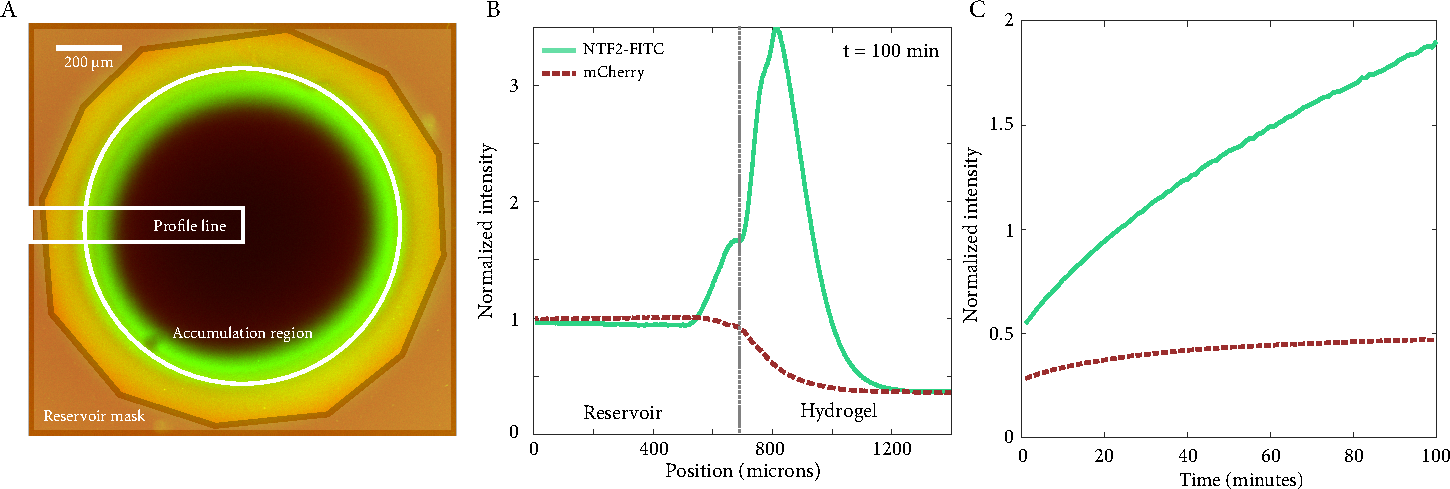
\includegraphics[width=\textwidth]{figs/ch04/influx-plots.pdf}
\label{fig:influx-plots}
\end{figure}

After recording a time series of fluorescent protein influx into a hydrogel, diffusion constants can be estimated using either a plot of the intensity profile across the gel or a plot of total accumulation within the gel.  Figure~\ref{fig:influx-plots} shows an example of each plot.  The intensity within the gel is normalized to the average intensity of the reservoir, as calculated using the mask shown in Fig~\ref{fig:influx-plots}A.  Therefore, each profile trace begins at $I=1$ within the reservoir and either dips or rises to the partition coefficient value within the gel.  As the gels are not equilibrated, much of the gel interior shows only background fluorescence.  Likewise, the average intensity within the hydrogel trends towards the partition coefficient but does not reach it on the time scale of an average experiment.

Analysis of the accumulation and profile curves used the diffusion-equation solutions described by Mortensen, Okkels, and Bruus \cite{mortensen06}.  This method assumes that the edge of  a nearly-circular two-dimensional region is held at a fixed concentration while the interior equilibrates (Fig.~\ref{fig:mortensen}.  Such boundary conditions correspond to an infinite fluorophore reservoir.  Given that our reservoirs are 10-20 times larger than the hydrogel volume, this is a reasonable assumption.  In a slight modification, we allow for an arbitrary partition coefficient $\gamma$ by taking the fixed boundary concentration $c_0$ to be $\gamma T_0$, where $T_0$ is the fluorescent protein intensity in the reservoir.  The assumption of near-circularity is also a good one.

\begin{SCfigure}
\caption{Geometry used to solve diffusion equation in \cite{mortensen06}.  The reservoir concentration $c_0$ fixed the concentration at the edge of the region $\Omega$.  The concentration $c(\mathbf{r},t)$ is determined within $\Omega$ as a function of position and time.}
\centering
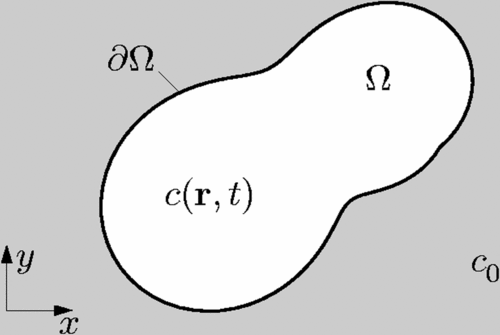
\includegraphics[width=0.4\textwidth]{figs/ch04/mortensen}
\label{fig:mortensen}
\end{SCfigure}

The two most troublesome restrictions of the Mortensen equations are Fickian diffusion and the homogeneity of the hydrogel.  As discussed in Sec.~\ref{sec:fickian}, the presence of the hydrogel meshwork and binding make diffusion within the hydrogels slightly anomalous.  Additionally, despite the improvements to the fabrication protocol, the hydrogels likely contain some degree of nonuniformity in their density, with the centers most likely being slightly denser than the edges due to differential swelling.  The effects of swelling and non-uniform thickness are greatest at the gel edge.  Unfortunately, the points at the edge of the gel and earliest in the experiment are the most important to the following fits.  As a result, the diffusion constants extracted using the profile and accumulation plots are not reliable.  The analysis is presented below nonetheless, as a similar approach was taken in analyzing the FRAP experiments.

\subsection{Profile analysis}
% figure  '180209_FSFG-gel_2.vsi'
\label{sec:profile-analysis}

Mortensen \textit{et al} first define a characteristic timescale for equilibration $\tau = (\mathcal{A}/\mathcal{P})^2 (\pi/4D)$ where $\mathcal{A}$ and $\mathcal{P}$ are the area and perimeter, respectively, of $\Omega$.  For a circle $\mathcal{A}/\mathcal{P} = a/2$, but this ratio was numerically calculated for the hydrogels (Sec.~\ref{sec:gel-dim}).  For times $t \ll \tau$, the concentration profile as a function of the distance $r$ from the gel center can be approximated as 
\begin{equation}
c(r,t) = c_0 \,\mathrm{erfc}\left(\frac{r}{\sqrt{4Dt}}\right)
\label{eq:approx-profile}
\end{equation}
where $D$ is the diffusion constant.

%% erfc position at fixed time '180525_FSFGPEGDA700_03.vsi'
%% t is close to beginning but not right at beginning

\begin{figure}
\caption{IFits to Eqn.~\ref{eq:approx-profile} near the beginning of the influx experiment for (A) mCherry and (B) NTF2-Alexa488 intensity profiles.  Hydrogel nominally contains 10 mg/mL FSFG-PEGDA 700 kDa.  The entire intensity profile is shown in the top panel with the portion used for fitting highlighted in red.  Approximate locations of the gel edge, background fluoresence level, and partition coefficient are also shown.}
\centering
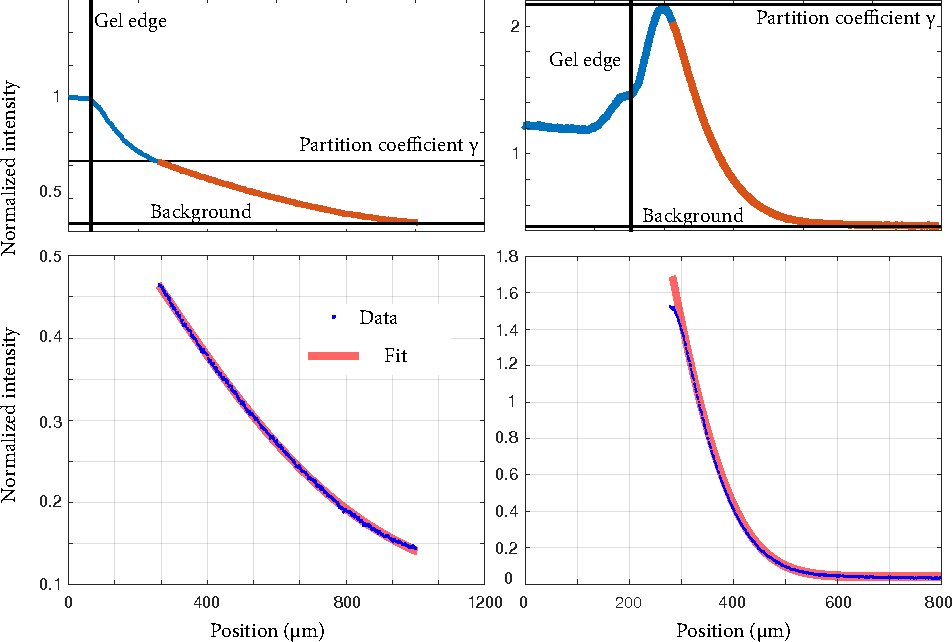
\includegraphics[width=0.9\textwidth]{figs/ch04/erfc-position.pdf}
\label{fig:erfc-position}
\end{figure} 

\begin{SCfigure}
\caption{Fits to Eqn.~\ref{eq:approx-profile} at a fixed point near the gel edge for (A) mCherry and (B) NTF2-Alexa488 intensity profiles.  The short-time approximation likely only holds for times $t \lesssim 20$ minutes. Hydrogel nominally contains 10 mg/mL FSFG-PEGDA 700 kDa.\\}
\centering
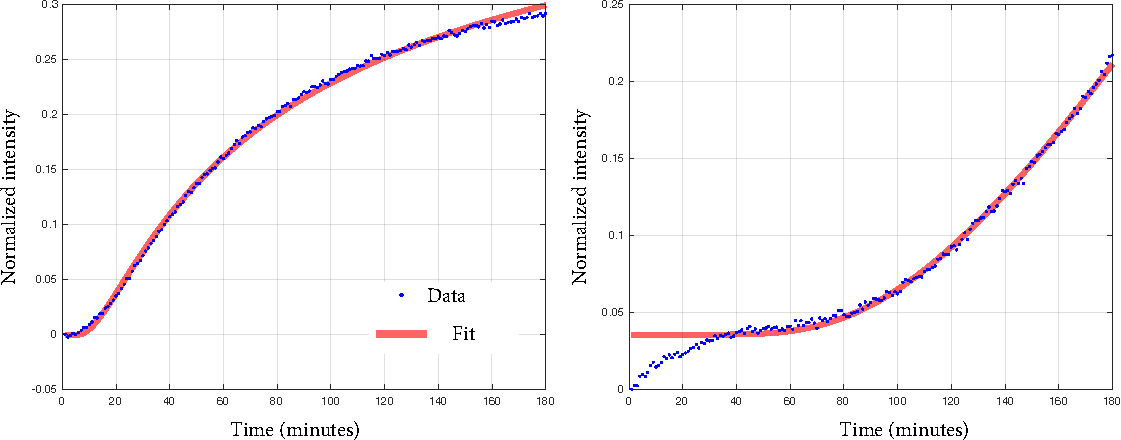
\includegraphics[width=0.7\textwidth]{figs/ch04/erfc-time.pdf}
\label{fig:erfc-time}
\end{SCfigure} 

The typical duration of an influx experiment was approximately $\tau$, making the short-time approximation questionable throughout most of the time series.  We attempted to fit the intensity profile (Fig.~\ref{fig:erfc-position}) and obtained fits with fairly low error but with unreliable fit parameters.  In addition to the issues of timescale, it was often difficult to determine where the gel edge was located, as well as the partition coefficient.  Given these problems, it is not surprising that fits at successive timepoints yielded incompatible values of diffusion constant for both mCherry and NTF2.  A similar problem prevented the use of diffusion constants obtained from intensity fits at a fixed position over time (Fig.~\ref{fig:erfc-time}).

A more exact solution for $c(r,t)$ can be written if the gel is assumed to be circular.  Mortensen \textit{et al} quantify the error introduced by small deviations from circularity and find it to be small.  Assuming a circular gel, the concentration profile at an arbitrary time $t$ is given by
\begin{equation}
\frac{c(r,t)}{c_0} = 1 - 2\sum_{n=0}^\infty \frac{J_0(\alpha_n r)}{\alpha_n a J_1(\alpha_n a)}\exp(-\alpha_n D t)
\label{eq:full-profile}
\end{equation}
where $a$ is the gel radius and $\alpha_n a$ is the $n$th zero of the Bessel function of the first kind $J_0$.

I fit the intensity profiles to Eqn.~\ref{eq:full-profile} using different numbers of terms $N$.  For the mCherry curves, the resulting fit parameters tended to converge as $N$ increased, and the RMSE stabilized.  However, neither was true for the NTF2 curves.  Increasing values of $N$ led to steadily decreasing values of diffusion constant.  This may be due to the effect of binding on NTF2 diffusion.

\subsection{Accumulation analysis}

The total accumulation within the hydrogel can be modeled by integrating the concentration profile over the entire gel.  When this is done, the averaged intensity within the hydrogel $N(t)$ is found to be
\begin{equation}
\frac{N(t)}{N_0} = 1-\sum_{n=0}^\infty \frac{4}{(\alpha_na)^2}\exp\left(-\frac{(\alpha_na)^2\pi t}{16\tau}\right)
\label{eq:full-accumulation}
\end{equation} where$N_0$ is the equilibrium value, here equal to the partition coefficient $\gamma$ once the intensity has been normalized to that of the reservoir.

\begin{SCfigure}
\caption{Accumulation fits to Eqn.~\ref{eq:full-accumulation} for (A) mCherry and (B) NTF2-Alexa488.  Hydrogel nominally contains 10 mg/mL FSFG-PEGDA 700 kDa.\\}
\centering
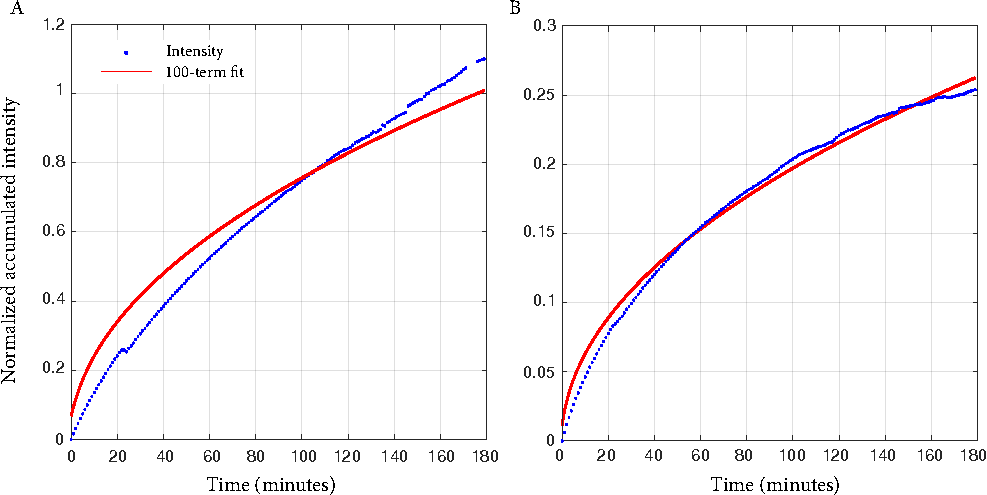
\includegraphics[width=0.7\textwidth]{figs/ch04/accumulation.pdf}
\label{fig:acc}
\end{SCfigure} 

% figure ''180516-FSFGbis_2.vsi'' fit to 100 terms, made with processing-4 script, results 11-12-18.mat

Fits to the first 100 terms of Eqn.~\ref{eq:full-accumulation} are shown in Fig.~\ref{fig:acc} for mCherry and NTF2.  These fits had systematic error, likely for the same reasons as the profile fits.

While the profile and accumulation data do contain information on the diffusion constants of NTF2 and mCherry, I was unable to reliably extract that information using the influx experiments.  The model presented above is a remarkably good match to the experimental setup except for the presence of binding and the unpredictable gel-edge effects.  The FRAP experiments overcome the problem of edge effects by making use of equilibrated regions deep within the hydrogel.

\section{FRAP analysis}
\label{sec:FRAP-analysis}



\subsection{Accounting for photobleaching}
Small but noticeable amounts of photobleaching occur over the course of the FRAP experiment.  In order to correct for photobleaching, the intensity of the bleached spot must be normalized to that of the entire gel, including the bleached region.  The normalized intensity used to fit the recovery curves is given by
\begin{equation}
N(t) = \frac{c_b(t)}{c_g(t)}
\end{equation} where the average intensity within the bleach spot is $c_b(t) = C_b(t)/A_b$ is the total intensity $C_b(t)$ within the bleach spot and $A_b$ is the area of the spot.  The average intensity within the gel $c_g(t)$ is defined similarly.  Using this normalization removes the effects of photobleaching, as verified by simulating recovery data with various photobleaching rates (Loren did this, I might have a copy of the code).
\subsection{No-exchange analysis}
A simple analysis of the recovery curve assumes that there is no exchange of transport factor or inert protein between the reservoir and the hydrogel, only between bleached and unbleached portions of the hydrogel.  It further assumes a uniform hydrogel which is completely equilibrated.  If those things are true, the normalized intensity within the bleach spot over time can be written as
\begin{equation}
N(t) = A\exp(-\tau/2t)\left(\mathrm{I}_0(\tau/2t)+\mathrm{I}_1(\tau/2t)\right)+C
\end{equation}

\subsection{Fourier transform solution}

We have the problem that our gels are not perfectly equilibrated, and that they exchange with the reservoir.  In order to solve that problem, we analyzed the data using a model from the heat transfer book.  This solution makes use of Green's functions and a 2D polar Fourier transform.  We assume the gel is a circle and constrain the edge of the circle to be at zero concentration.  Then we build up the mode coefficients using the initial post-bleach intensity distribution and use them to predict the time-evolution of the system.  The overall solution is given by
\begin{equation}
c(r,\theta,t) = C\sum_{n=-\infty}^{\infty} \sum_{\alpha = 0}^\infty   \frac{\exp\left(-D\alpha^2t\right)\mathrm{J}_n\left(\alpha r\right)}{\left(\mathrm{J'}_n(\alpha a)\right)^2} \int_0^{2\pi} \int_0^a \cos\left(n(\theta-\theta')\right) \mathrm{J}_n(\alpha r') f(r',\theta') r' dr' d\theta'
\end{equation}
Looking at just the integral part, we can rewrite it using a trig identity to separate the primed and unprimed coordinates.  The solution can then be written
\begin{eqnarray}
c(r,\theta,t) &=& \sum_{n=-\infty}^{\infty} \sum_{\alpha = 0}^\infty   \frac{\exp\left(-D\alpha^2t\right)\mathrm{J}_n\left(\alpha r\right)}{\left(\mathrm{J'}_n(\alpha a)\right)^2} \left(c_{n,\alpha}\cos(n\theta') + s_{n,\alpha} \sin(n\theta')\right) \\
c_{n,\alpha} & = &b_{n,\alpha} \int_0^{2\pi} \int_0^a \cos\left(n\theta'\right) \mathrm{J}_n(\alpha r')f(r',\theta') r' dr' d\theta'\\
s_{n,\alpha} & = & b_{n,\alpha}\int_0^{2\pi} \int_0^a \sin\left(n\theta'\right) \mathrm{J}_n(\alpha r') f(r',\theta') r' dr' d\theta'
\end{eqnarray}
In order to implement this computationally, I actually integrate over the whole image but mask the parts that aren't in the gel.  I set the coordinate system to 

\section{Discussion}